\documentclass[11pt,a4paper]{article}

\usepackage[left=2.4cm,right=2.4cm,top=2.2cm,bottom=2.2cm]{geometry}

\usepackage[T1]{fontenc}
\usepackage[utf8]{inputenc}
\usepackage{newtxtext,newtxmath}
\usepackage{microtype}

\usepackage{amsmath}
\usepackage{booktabs}
\usepackage{siunitx}
\usepackage{graphicx}
\graphicspath{{figures/}{./}}
\usepackage{enumitem}
\usepackage{xcolor}
\newcommand{\redflag}[1]{\textcolor{red}{[#1]}}

\usepackage[hidelinks]{hyperref}

\sisetup{
  detect-weight = true,
  detect-family = true
}

% Supplementary numbering
\renewcommand{\thetable}{S\arabic{table}}
\renewcommand{\thefigure}{S\arabic{figure}}
\renewcommand{\theequation}{S\arabic{equation}}

\setcounter{secnumdepth}{3}

% Paragraph and line spacing
\setlength{\parindent}{0pt}
\setlength{\parskip}{0.35\baselineskip}
\linespread{1.03}

\begin{document}

\begin{center}
{\Large\bfseries Supplementary Information\par}

\vspace{0.7em}

{\large\bfseries
Physics as the label for measuring and correcting materials reasoning in multimodal models
\par}

\vspace{0.8em}

{\normalsize
Hasan Kurban, Rasul Khanbayov, and Mustafa Kurban
\par}
\end{center}

\vspace{1.0em}

\noindent
This Supplementary Information contains Supplementary Note 1, which provides
the standard derivations underlying the physical oracles and statistical
estimators used in the Article; Supplementary Note 2, which records how the oracle
definitions and the verifier split reached the final form used for every reported result;
Supplementary Figure S1 (full precision-audit breakdown); and Supplementary Tables S1--S6: per-cell
PCR with bootstrap intervals (S1), coverage and alternative treatments of non-checkable responses
(S2), paired multiplicity-corrected model comparisons (S3), class-conditional DFT rates (S4), the
violation taxonomy for the spectrum and DFT families (S5), the common class-balanced DFT item
set (S6), stability results under the original and final stability rules (S7), and the second-annotator and
oracle-silent audits (S8). Proposition~1 and Corollary~1, which constitute the main
measurement-theoretic result of the study, are stated and proved in the main
Article.

\vspace{0.5em}

\section*{Supplementary Note 1: standard derivations}
\noindent The results collected here are standard and are included for completeness.
\setcounter{subsection}{0}
\renewcommand{\thesubsection}{1.\arabic{subsection}}

\subsection{Bragg's law and \texorpdfstring{$d$}{d}-spacing}
For constructive interference from lattice planes of spacing $d$ at Bragg angle
$\theta$ with a beam of wavelength $\lambda$, the path difference $2d\sin\theta$ equals an
integer number of wavelengths; for first order ($n=1$), $\lambda=2d\sin\theta$. The
measured scattering angle is $2\theta$, so a claimed peak at $2\theta$ corresponds to
$d=\lambda/\!\big(2\sin\theta\big)$ with $\theta$ equal to half the measured angle.
Physical realizability requires $\sin\theta\le1$, equivalently $d\ge\lambda/2$, and the
instrument range further restricts $2\theta$ to a finite window; the diffraction oracle
enforces both and matches claimed peaks to the reference pattern of the stated phase
within tolerance.

\subsection{Scale-bar calibration}
A scale bar of stated length $\ell_{\mathrm{nm}}$ spanning $p_{\mathrm{bar}}$ pixels
fixes the calibration $s=\ell_{\mathrm{nm}}/p_{\mathrm{bar}}$ (nanometres per pixel).
For an image whose long edge is $p_{\mathrm{img}}$ pixels, the field of view is
$s\,p_{\mathrm{img}}$ nanometres, which upper-bounds any reported feature size and
defines the microscopy oracle.

\subsection{Convex-hull stability}
For a given composition, the energy above the convex hull $E_{\mathrm{hull}}\ge0$ is the
formation energy minus that of the lowest-energy combination of stable phases at the
same composition. A phase is thermodynamically stable when $E_{\mathrm{hull}}=0$ and is
treated as within tolerance when $E_{\mathrm{hull}}\le\epsilon$; the DFT-grounded near-hull oracle uses the reported threshold
$\epsilon=0.05\,\mathrm{eV\,atom^{-1}}$.

\subsection{Percentile bootstrap confidence intervals}
For a rate estimated from $n$ items we resample items with replacement $B$ times,
recompute the rate on each resample, and report the empirical $\alpha/2$ and
$1-\alpha/2$ quantiles. Under independent sampling of items the interval is consistent
as $n,B\to\infty$. Where items share a parent source (for example, several questions
about one structure), we resample at the source level to respect that dependence. We
report the interval for all rates.

\subsection{Concentration of the empirical rate}
For a rate $\bar X=\frac1n\sum_{i=1}^n X_i$ that averages independent variables
$X_i\in[0,1]$ with mean $\mathbb{E}[\bar X]=\mu$, Hoeffding's inequality gives
$\Pr[\,|\bar X-\mu|>t\,]\le 2e^{-2nt^2}$ for every $t>0$. Applied to $X_i=1-Y_i$ this
bounds the sampling error of $\mathrm{PCR}^\star$ about the population physical-consistency rate; where items share a parent source, $n$ is the number of independent sources, matching the source-level percentile bootstrap above.

\subsection{Exact McNemar test}
For paired before/after consistency, let $b$ and $c$ be the numbers of discordant items
(consistent-then-inconsistent, i.e.\ regressions, and inconsistent-then-consistent,
i.e.\ fixes). Under the null that each discordant item changes direction with
probability $\tfrac12$, $c\sim\mathrm{Binomial}(b+c,\tfrac12)$, and the two-sided exact
$p$-value is $\min\!\big(1,\,2\sum_{k=0}^{\min(b,c)}\binom{b+c}{k}2^{-(b+c)}\big)$. This
is the test used for CGSV in the main Article.
\subsection{Distribution-free bound on the total error of a reported rate}
The main Article's Proposition~1 and Corollary~1 are exact statements about the oracle's
bias on a fixed set of items. If, in addition, the checkable items are drawn independently
from the benchmark's item-generating process, with
$\mu=\mathbb{E}[1-Y_i]$ that process's physical-consistency rate, then splitting
$\mathrm{PCR}-\mu=(\mathrm{PCR}-\mathrm{PCR}^\star)+(\mathrm{PCR}^\star-\mu)$, bounding the
first term by $(1-\hat d)+\hat f$ (Corollary~1) and the second by the concentration
inequality above gives, for every $t>0$, with probability at least $1-2e^{-2nt^2}$,
\[
|\mathrm{PCR}-\mu|\;\le\;\underbrace{(1-\hat d)+\hat f}_{\text{oracle bias}}\;+\;\underbrace{t}_{\text{sampling}}.
\]
Where items share a parent source the same statement holds with $n$ replaced by the number
$m$ of independent sources under balanced source sizes; unequal sizes give a size-weighted
mean and a correspondingly weaker rate. Both steps are standard, and the independence
assumption is an idealization for a convenience benchmark. At the cell sizes used in the
Article the sampling term is far looser than the percentile bootstrap interval: at $n=90$ and
$95\%$ confidence it is $t=0.143$, against reported per-cell intervals of roughly $\pm0.09$.
The Article therefore reports bootstrap intervals as its uncertainty and uses this bound only
to show that the two sources of error are separately controlled.

\clearpage
\section*{Supplementary Figure S1}
\noindent\textbf{Oracle precision audit, every family, full breakdown.} Referenced from
the main Article's Results (Oracle validity subsection). Each bar is every
human-reviewed oracle-fired case for that family (Article, Table~1), split into real
violations, false positives, and unsure verdicts, as judged by the first annotator. Single-annotator precision
is 77.2--95.3\% (the stability bar shows the original audit of 107 cases, of which the 57 scored under the final
stability rule are all genuine violations, Article Table~1) but not uniform: diffraction's tolerance is visibly the tightest relative
to typical model precision, while the three DFT-grounded families cluster above 92\%. After a second annotation and
adjudication, consensus precision is lower for diffraction and spectra (0.60 and 0.61) and essentially unchanged for
the other families (Article Table~1; Supplementary Table~S8).
\begin{figure}[htbp]
\centering
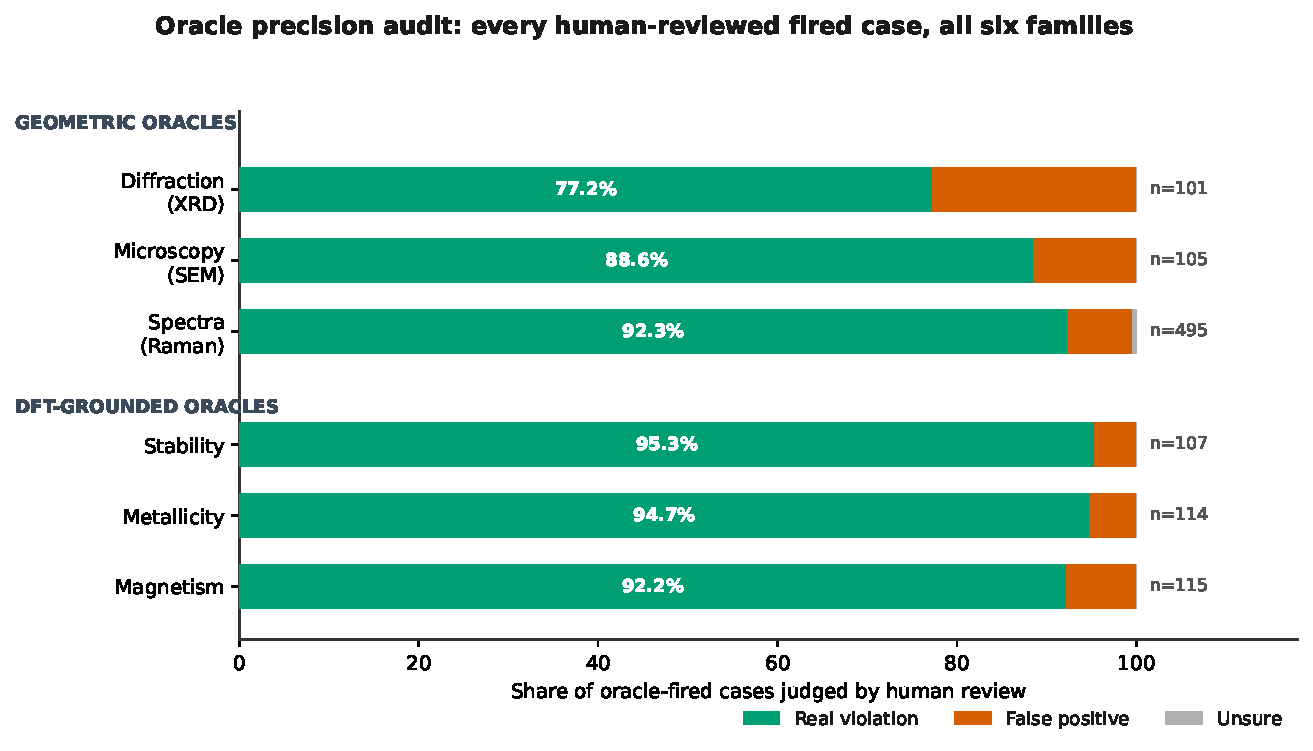
\includegraphics[width=0.92\linewidth]{fig_precision_funnel.pdf}
\label{fig:precision-funnel}
\end{figure}

\clearpage
\section*{Supplementary Table S1}
\noindent\textbf{Per-cell Physical-Consistency Rate with bootstrap 95\% confidence
intervals.} Referenced from the main evaluation table of the Article. $n$ is the number of checkable records in the cell
(pooled across $S=3$ seeds); CI is the percentile bootstrap 95\% interval ($B=10{,}000$
resamples) on the cell's own PCR. The first four models are the originally evaluated set;
the next four are the later-generation refresh; the last (GPT-5.6-Sol) is a flagship-tier
addition testing whether it exceeds the balanced-tier GPT-5.6-Terra within the same
generation (Article, Table~1 note). Each item in this benchmark exposes
exactly one checkable constraint of its own constraint type, so the per-constraint-type
violation rate $\rho_t=1-\mathrm{PCR}$ for every cell below and is not tabulated separately. Stability rows use
the final stability oracle, which does not score near-hull materials; the original rule's values are in
Table~S7.
\begin{table}[htbp]
\centering
{\scriptsize\setlength{\tabcolsep}{4pt}\renewcommand{\arraystretch}{1.05}
\begin{tabular}{l l S[table-format=3.0] S[table-format=1.3] c}
\toprule
Model & Constraint type & {$n$} & {PCR} & {95\% CI} \\
\midrule
Qwen2.5-VL-7B & Diffraction & 64 & 0.500 & [0.375, 0.625] \\
Qwen2.5-VL-7B & Microscopy & 87 & 0.667 & [0.563, 0.759] \\
Qwen2.5-VL-7B & Spectra & 88 & 0.148 & [0.080, 0.227] \\
Qwen2.5-VL-7B & Stability$^{*}$ & 72 & 0.917 & [0.847, 0.972] \\
Qwen2.5-VL-7B & Metallicity$^{*}$ & 87 & 0.540 & [0.437, 0.644] \\
Qwen2.5-VL-7B & Magnetism$^{*}$ & 90 & 0.767 & [0.678, 0.856] \\
\addlinespace
Gemini 2.5 Flash Lite & Diffraction & 60 & 0.517 & [0.400, 0.650] \\
Gemini 2.5 Flash Lite & Microscopy & 86 & 1.000 & [1.000, 1.000] \\
Gemini 2.5 Flash Lite & Spectra & 90 & 0.278 & [0.189, 0.378] \\
Gemini 2.5 Flash Lite & Stability$^{*}$ & 70 & 0.814 & [0.729, 0.900] \\
Gemini 2.5 Flash Lite & Metallicity$^{*}$ & 84 & 0.702 & [0.607, 0.798] \\
Gemini 2.5 Flash Lite & Magnetism$^{*}$ & 89 & 0.494 & [0.382, 0.596] \\
\addlinespace
GPT-4o & Diffraction & 64 & 0.625 & [0.500, 0.750] \\
GPT-4o & Microscopy & 87 & 0.954 & [0.908, 0.989] \\
GPT-4o & Spectra & 44 & 0.068 & [0.000, 0.159] \\
GPT-4o & Stability$^{*}$ & 79 & 0.886 & [0.810, 0.949] \\
GPT-4o & Metallicity$^{*}$ & 85 & 0.671 & [0.565, 0.765] \\
GPT-4o & Magnetism$^{*}$ & 90 & 0.678 & [0.578, 0.778] \\
\addlinespace
Claude Sonnet 4.5 & Diffraction & 64 & 0.547 & [0.422, 0.672] \\
Claude Sonnet 4.5 & Microscopy & 87 & 0.977 & [0.943, 1.000] \\
Claude Sonnet 4.5 & Spectra & 90 & 0.189 & [0.111, 0.267] \\
Claude Sonnet 4.5 & Stability$^{*}$ & 73 & 0.849 & [0.767, 0.931] \\
Claude Sonnet 4.5 & Metallicity$^{*}$ & 85 & 0.694 & [0.600, 0.788] \\
Claude Sonnet 4.5 & Magnetism$^{*}$ & 90 & 0.756 & [0.666, 0.844] \\
\addlinespace
Claude Opus 4.6 & Diffraction & 64 & 0.578 & [0.453, 0.703] \\
Claude Opus 4.6 & Microscopy & 87 & 0.954 & [0.908, 0.989] \\
Claude Opus 4.6 & Spectra & 90 & 0.244 & [0.156, 0.333] \\
Claude Opus 4.6 & Stability$^{*}$ & 76 & 0.789 & [0.697, 0.882] \\
Claude Opus 4.6 & Metallicity$^{*}$ & 86 & 0.721 & [0.628, 0.814] \\
Claude Opus 4.6 & Magnetism$^{*}$ & 90 & 0.700 & [0.600, 0.789] \\
\addlinespace
GPT-5.6-Terra & Diffraction & 64 & 0.797 & [0.703, 0.891] \\
GPT-5.6-Terra & Microscopy & 81 & 0.951 & [0.901, 0.988] \\
GPT-5.6-Terra & Spectra & 90 & 0.833 & [0.756, 0.911] \\
GPT-5.6-Terra & Stability$^{*}$ & 75 & 0.653 & [0.547, 0.760] \\
GPT-5.6-Terra & Metallicity$^{*}$ & 85 & 0.659 & [0.553, 0.753] \\
GPT-5.6-Terra & Magnetism$^{*}$ & 90 & 0.767 & [0.678, 0.844] \\
\addlinespace
Qwen3-VL-8B-Instruct & Diffraction & 62 & 0.468 & [0.355, 0.597] \\
Qwen3-VL-8B-Instruct & Microscopy & 86 & 0.802 & [0.709, 0.884] \\
Qwen3-VL-8B-Instruct & Spectra & 90 & 0.133 & [0.067, 0.200] \\
Qwen3-VL-8B-Instruct & Stability$^{*}$ & 75 & 0.747 & [0.653, 0.840] \\
Qwen3-VL-8B-Instruct & Metallicity$^{*}$ & 77 & 0.688 & [0.584, 0.792] \\
Qwen3-VL-8B-Instruct & Magnetism$^{*}$ & 90 & 0.533 & [0.433, 0.633] \\
\addlinespace
Qwen3-VL-8B-Thinking & Diffraction & 64 & 0.578 & [0.453, 0.703] \\
Qwen3-VL-8B-Thinking & Microscopy & 87 & 0.885 & [0.816, 0.943] \\
Qwen3-VL-8B-Thinking & Spectra & 87 & 0.092 & [0.034, 0.161] \\
Qwen3-VL-8B-Thinking & Stability$^{*}$ & 76 & 0.895 & [0.816, 0.961] \\
Qwen3-VL-8B-Thinking & Metallicity$^{*}$ & 87 & 0.644 & [0.540, 0.736] \\
Qwen3-VL-8B-Thinking & Magnetism$^{*}$ & 89 & 0.506 & [0.404, 0.607] \\
\addlinespace
GPT-5.6-Sol & Diffraction & 61 & 0.820 & [0.721, 0.918] \\
GPT-5.6-Sol & Microscopy & 82 & 0.915 & [0.854, 0.976] \\
GPT-5.6-Sol & Spectra & 89 & 0.764 & [0.674, 0.854] \\
GPT-5.6-Sol & Stability$^{*}$ & 71 & 0.789 & [0.690, 0.887] \\
GPT-5.6-Sol & Metallicity$^{*}$ & 88 & 0.670 & [0.580, 0.761] \\
GPT-5.6-Sol & Magnetism$^{*}$ & 90 & 0.733 & [0.644, 0.822] \\
\bottomrule
\end{tabular}}
\end{table}

\clearpage
\section*{Supplementary Note 2: development history of the oracles and the verifier split}
Every result in the Article uses the final oracle definitions and the source-disjoint verifier
split described in its Methods. This note records the earlier versions, so that numbers in
earlier drafts or in the public repository history can be reconciled with the Article.

\paragraph{Spectrum oracle.} The first spectrum oracle accepted a claimed peak if a windowed maximum
of sufficient prominence lay near it. A first precision audit of that version (72.8\%, $n=103$)
showed that the criterion did not match human judgement of a peak on noisy, baseline-drifting
Raman spectra, because a monotonic rise or a shoulder could satisfy it. The oracle was revised to
require a genuine interior local maximum (Methods). The collected Half-B responses were re-scored
with the revised oracle and the resulting 495 fired cases re-audited (92.7\%; Article, Table~1).
The main evaluation, the accuracy-versus-consistency analysis and the CGSV experiment were re-run
under the revised oracle. Spectra PCR fell for every model, the mean accuracy--consistency
disagreement changed from 41.8\% to 22.2\% (23.6\% on the diffraction and spectra cells under the final
stability rule, on which the stability arm shows no disagreement), and the CGSV experiment changed from 555 to 545
checkable records.

\paragraph{Magnetism oracle.} The first magnetization check compared the computed reference with zero
using exact floating-point equality, which misfired on 82 of 3{,}000 materials whose computed
magnetization was near but not exactly zero. It was first patched with a $10^{-6}\,\mu_{\mathrm{B}}$
tolerance and then, following the domain co-author's review of the DFT protocol, replaced by the
per-atom classification at $0.05\,\mu_{\mathrm{B}}\,\mathrm{atom}^{-1}$ that never compares sign. The same
review introduced the metallicity abstention band and the near-hull wording for stability. The DFT
Half-B responses were re-collected under the final definitions before the audit reported in Table~1.

\paragraph{Stability abstention band.} The original stability oracle required a STABLE claim whenever
$E_{\mathrm{hull}}\le0.05$~eV\,atom$^{-1}$, while the stability prompt tells the model to treat any borderline or
metastable case as UNSTABLE. A model following the prompt on a near-hull material was therefore counted as a
violation. This conflict was found during revision, when a second, independent annotator re-labelled a subsample of
the stability audit: all 13 disagreements with the first annotator were UNSTABLE claims on near-hull materials.
The final oracle does not score $0<E_{\mathrm{hull}}\le0.05$ (abstention band, as for metallicity). The change affects
89 flagged records in the main evaluation and 50 of the 107 audited stability cases; all stability-dependent numbers
in the Article were recomputed from the collected responses, without new model calls, and the original rule's
values are given in Table~S7. The verifier was trained on labels from the original rule; evaluated on the test items
the final rule scores, its in-distribution AUC is 0.871 (stability family 0.911) and its held-out stability AUC 0.372.
The prompt-paraphrase sensitivity check for stability (Article, Methods) did not retain per-item claims and is
reported under the original rule. The stability row of Table~S5 was computed on the original audit's 102 real
violations, 45 of which are near-hull.

\paragraph{Materials Project retrievals.} The precision-audit sample used a retrieval of database
version 2026.04.13 on 2026-07-16; the reported evaluation used a retrieval of the same version on
2026-08-05. All 210 audited materials appear with the same identifiers in the later batch.

\paragraph{Verifier split.} The first in-distribution split was drawn at the record level, so records
from the same source item (seed replicates, different models' claims) could fall on both sides. It
gave an in-distribution AUC of 0.858 and a held-out magnetism AUC of 0.867, which earlier drafts of
this work reported as an exception to the lack of transfer. Under the source-disjoint split used in the
Article, the in-distribution AUC is 0.850 and held-out magnetism is 0.503, at chance; the exception
was an artifact of the leak and is withdrawn. The verifier dataset changed from 2{,}416 to 2{,}152
records when the spectrum records were re-scored with the revised oracle.

\paragraph{Violation taxonomy.} The diffraction and microscopy taxonomy (Article, Fig.~1c) was
computed before the spectrum and DFT audits had been redone under the final oracles; the taxonomy
for those four families (Table~S5) was computed on the final audits during revision.

\paragraph{Verifier weights.} The original training script did not save the adapter weights. The
script was corrected and all 13 adapters were retrained for release (seed 0; float32 on an NVIDIA
P100, because that GPU lacks bfloat16 support); the released adapters reproduce the in-distribution result of the Article's verifier table (Table~5)
exactly (AUC 0.850, 95\% CI [0.814, 0.884]; $F_1$ 0.737 vs.\ 0.735). Held-out AUCs move by up to 0.08:
diffraction 0.532 (reported 0.497), microscopy 0.602 (0.527; Bonferroni-corrected interval
[0.519, 0.682], above chance), spectra 0.536 (0.558), stability 0.383 (0.436; below chance), metallicity
0.542 (0.582) and magnetism 0.502 (0.503). The held-out results are thus sensitive to the training run,
while the conclusion that no held-out family transfers at a useful level holds for both runs.

% generated by experiments/exp31_si_tables.py -- do not edit by hand
\clearpage
\section*{Supplementary Table S2}
\noindent\textbf{Coverage of the Physical-Consistency Rate and alternative treatments of non-checkable
responses.} Each (model, constraint-type) cell attempts 90 items (30 per seed, $S=3$). Items the
oracle can score (evaluable) per cell: diffraction 64; microscopy 87; spectra 90; stability 71--79; metallicity 82--89; magnetism 90. Diffraction items without a usable reference
structure, metallicity items in the 0.05--0.20~eV abstention band and near-hull stability materials
($0<E_{\mathrm{hull}}\le0.05$~eV\,atom$^{-1}$) are not evaluable for any model.
For image constraint types an item counts as evaluable if at least one of the nine models produced a
checkable response on it (all models received the same items), which is a lower bound on true
evaluability. Coverage is checkable responses / evaluable items; it absorbs the rare API failures and
time-outs, which the result files do not record separately. Overall PCR (rank in parentheses) under
three conventions: \emph{excluded} (reported in the Article; non-checkable responses are not scored),
\emph{penalised} (a non-checkable response counts as a violation) and \emph{lenient} (it counts as
consistent). Kendall $\tau$ of the model ordering against the reported convention: penalised
0.83, lenient 1.00.
\begin{table}[htbp]
\centering
{\scriptsize\setlength{\tabcolsep}{3.2pt}\renewcommand{\arraystretch}{1.08}
\begin{tabular}{l cccccc ccc}
\toprule
& \multicolumn{6}{c}{Coverage} & \multicolumn{3}{c}{Overall PCR (rank)} \\
\cmidrule(lr){2-7}\cmidrule(lr){8-10}
Model & Diffr. & Micro. & Spectra & Stab. & Metal. & Magn. & excluded & penalised & lenient \\
\midrule
Qwen2.5-VL-7B & 1.00 & 1.00 & 0.98 & 1.00 & 1.00 & 1.00 & 0.584 (8) & 0.582 (8) & 0.586 (8) \\
Gemini 2.5 Flash Lite & 0.94 & 0.99 & 1.00 & 0.99 & 0.97 & 0.99 & 0.630 (6) & 0.618 (6) & 0.638 (6) \\
GPT-4o & 1.00 & 1.00 & 0.49 & 1.00 & 1.00 & 1.00 & 0.699 (3) & 0.634 (5) & 0.727 (3) \\
Claude Sonnet 4.5 & 1.00 & 1.00 & 1.00 & 1.00 & 1.00 & 1.00 & 0.667 (4) & 0.667 (3) & 0.667 (4) \\
Claude Opus 4.6 & 1.00 & 1.00 & 1.00 & 1.00 & 1.00 & 1.00 & 0.663 (5) & 0.663 (4) & 0.663 (5) \\
GPT-5.6-Terra & 1.00 & 0.93 & 1.00 & 1.00 & 1.00 & 1.00 & 0.777 (2) & 0.768 (1) & 0.780 (2) \\
GPT-5.6-Sol & 0.95 & 0.94 & 0.99 & 0.99 & 0.99 & 1.00 & 0.778 (1) & 0.760 (2) & 0.783 (1) \\
Qwen3-VL-8B-Instruct & 0.97 & 0.99 & 1.00 & 0.97 & 0.94 & 1.00 & 0.556 (9) & 0.545 (9) & 0.565 (9) \\
Qwen3-VL-8B-Thinking & 1.00 & 1.00 & 0.97 & 1.00 & 1.00 & 0.99 & 0.594 (7) & 0.589 (7) & 0.597 (7) \\
\bottomrule
\end{tabular}}
\end{table}

\clearpage
\section*{Supplementary Table S3}
\noindent\textbf{Paired, multiplicity-corrected model comparisons.} Differences are PCR of model A minus
model B. Image constraint types: all models answered the same items, so A and B are compared on the
items both answered checkably (exact McNemar test). DFT constraint types: models answered different
materials (Fisher's exact test). Overall: bootstrap of the difference that resamples paired items
jointly and DFT items within model ($B=10{,}000$; two-sided bootstrap $p$). 95\% CI: bootstrap.
MDE: smallest difference detectable with 80\% power at $\alpha=0.05$, $(z_{0.975}+z_{0.80})\times$
bootstrap SE. $p_{\mathrm{Holm}}$: Holm-corrected within the family shown. (a) The 12 comparisons
stated in the Article. (b) Within each constraint type, all 36 pairs: number significant after Holm
and median MDE. (c) All 36 pairs on overall PCR, ordered by $|\Delta|$.
\begin{table}[htbp]
\centering
{\scriptsize\setlength{\tabcolsep}{3pt}\renewcommand{\arraystretch}{1.05}
\begin{tabular}{l l r c r l r r}
\toprule
Comparison (A vs B) & Scope & $\Delta$ & 95\% CI & MDE & Test & $p$ & $p_{\mathrm{Holm}}$ \\
\midrule
\multicolumn{8}{l}{\itshape (a) Comparisons stated in the Article (Holm over 12)}\\
GPT-5.6-Terra vs GPT-4o & overall & +0.072 & [+0.018, +0.125] & 0.076 & bootstrap & 0.009 & 0.045 \\
Claude Opus 4.6 vs Claude Sonnet 4.5 & overall & -0.003 & [-0.050, +0.044] & 0.067 & bootstrap & 0.890 & 1.000 \\
Qwen3-VL-8B-Thinking vs Qwen3-VL-8B-Instruct & overall & +0.034 & [-0.016, +0.083] & 0.071 & bootstrap & 0.182 & 0.545 \\
GPT-5.6-Sol vs GPT-5.6-Terra & overall & +0.002 & [-0.042, +0.046] & 0.063 & bootstrap & 0.967 & 1.000 \\
Gemini 2.5 Flash Lite vs Qwen2.5-VL-7B & Microscopy & +0.326 & [+0.233, +0.430] & 0.143 & McNemar & $7.5\times10^{-9}$ & $8.9\times10^{-8}$ \\
GPT-4o vs Qwen2.5-VL-7B & Microscopy & +0.287 & [+0.184, +0.391] & 0.145 & McNemar & $4.2\times10^{-7}$ & $4.2\times10^{-6}$ \\
Claude Sonnet 4.5 vs Qwen2.5-VL-7B & Microscopy & +0.310 & [+0.218, +0.414] & 0.138 & McNemar & $1.5\times10^{-8}$ & $1.6\times10^{-7}$ \\
Claude Opus 4.6 vs Qwen2.5-VL-7B & Microscopy & +0.287 & [+0.184, +0.402] & 0.158 & McNemar & $4.6\times10^{-6}$ & $3.7\times10^{-5}$ \\
GPT-5.6-Terra vs Qwen2.5-VL-7B & Microscopy & +0.309 & [+0.198, +0.420] & 0.160 & McNemar & $1.6\times10^{-6}$ & $1.5\times10^{-5}$ \\
GPT-5.6-Sol vs Qwen2.5-VL-7B & Microscopy & +0.244 & [+0.122, +0.366] & 0.169 & McNemar & $3.2\times10^{-4}$ & 0.002 \\
Qwen3-VL-8B-Instruct vs Qwen2.5-VL-7B & Microscopy & +0.140 & [+0.023, +0.256] & 0.162 & McNemar & 0.029 & 0.116 \\
Qwen3-VL-8B-Thinking vs Qwen2.5-VL-7B & Microscopy & +0.218 & [+0.103, +0.333] & 0.162 & McNemar & $5.5\times10^{-4}$ & 0.003 \\
\bottomrule
\end{tabular}}

\vspace{0.8em}
{\scriptsize\setlength{\tabcolsep}{6pt}
\begin{tabular}{l r r}
\toprule
\multicolumn{3}{l}{\itshape (b) All 36 pairs within each constraint type (Holm over 36)}\\
Constraint type & significant pairs & median MDE \\
\midrule
Diffraction & 10 & 0.192 \\
Microscopy & 10 & 0.109 \\
Spectra & 15 & 0.149 \\
Stability & 3 & 0.175 \\
Metallicity & 0 & 0.202 \\
Magnetism & 9 & 0.194 \\
\bottomrule
\end{tabular}}
\end{table}
\begin{table}[htbp]
\centering
{\scriptsize\setlength{\tabcolsep}{3pt}\renewcommand{\arraystretch}{1.02}
\begin{tabular}{l l r c r l r r}
\toprule
\multicolumn{8}{l}{\itshape (c) All 36 pairs on overall PCR (Holm over 36): 18 significant}\\
Comparison (A vs B) & Scope & $\Delta$ & 95\% CI & MDE & Test & $p$ & $p_{\mathrm{Holm}}$ \\
\midrule
GPT-5.6-Terra vs Qwen3-VL-8B-Instruct & overall & +0.223 & [+0.169, +0.278] & 0.078 & bootstrap & $1.0\times10^{-4}$ & 0.004 \\
GPT-5.6-Sol vs Qwen3-VL-8B-Instruct & overall & +0.220 & [+0.165, +0.275] & 0.079 & bootstrap & $1.0\times10^{-4}$ & 0.004 \\
Qwen2.5-VL-7B vs GPT-5.6-Terra & overall & -0.198 & [-0.251, -0.144] & 0.076 & bootstrap & $1.0\times10^{-4}$ & 0.004 \\
GPT-5.6-Terra vs Qwen3-VL-8B-Thinking & overall & +0.189 & [+0.135, +0.243] & 0.077 & bootstrap & $1.0\times10^{-4}$ & 0.004 \\
Qwen2.5-VL-7B vs GPT-5.6-Sol & overall & -0.188 & [-0.242, -0.134] & 0.078 & bootstrap & $1.0\times10^{-4}$ & 0.004 \\
GPT-5.6-Sol vs Qwen3-VL-8B-Thinking & overall & +0.184 & [+0.129, +0.240] & 0.077 & bootstrap & $1.0\times10^{-4}$ & 0.004 \\
Gemini 2.5 Flash Lite vs GPT-5.6-Terra & overall & -0.151 & [-0.205, -0.098] & 0.076 & bootstrap & $1.0\times10^{-4}$ & 0.004 \\
Gemini 2.5 Flash Lite vs GPT-5.6-Sol & overall & -0.145 & [-0.200, -0.092] & 0.077 & bootstrap & $1.0\times10^{-4}$ & 0.004 \\
Claude Opus 4.6 vs GPT-5.6-Terra & overall & -0.118 & [-0.168, -0.067] & 0.073 & bootstrap & $1.0\times10^{-4}$ & 0.004 \\
Claude Opus 4.6 vs GPT-5.6-Sol & overall & -0.116 & [-0.168, -0.065] & 0.074 & bootstrap & $1.0\times10^{-4}$ & 0.004 \\
Claude Sonnet 4.5 vs GPT-5.6-Terra & overall & -0.115 & [-0.166, -0.063] & 0.074 & bootstrap & $1.0\times10^{-4}$ & 0.004 \\
Claude Sonnet 4.5 vs GPT-5.6-Sol & overall & -0.113 & [-0.165, -0.061] & 0.074 & bootstrap & $1.0\times10^{-4}$ & 0.004 \\
Claude Sonnet 4.5 vs Qwen3-VL-8B-Instruct & overall & +0.108 & [+0.059, +0.158] & 0.071 & bootstrap & $1.0\times10^{-4}$ & 0.004 \\
Claude Opus 4.6 vs Qwen3-VL-8B-Instruct & overall & +0.105 & [+0.052, +0.156] & 0.074 & bootstrap & $1.0\times10^{-4}$ & 0.004 \\
GPT-4o vs Qwen3-VL-8B-Instruct & overall & +0.098 & [+0.043, +0.153] & 0.077 & bootstrap & $2.0\times10^{-4}$ & 0.004 \\
Qwen2.5-VL-7B vs Claude Sonnet 4.5 & overall & -0.085 & [-0.137, -0.036] & 0.072 & bootstrap & 0.001 & 0.021 \\
Qwen2.5-VL-7B vs Claude Opus 4.6 & overall & -0.082 & [-0.133, -0.031] & 0.073 & bootstrap & 0.001 & 0.021 \\
GPT-4o vs GPT-5.6-Sol & overall & -0.081 & [-0.136, -0.029] & 0.077 & bootstrap & 0.004 & 0.065 \\
Claude Sonnet 4.5 vs Qwen3-VL-8B-Thinking & overall & +0.077 & [+0.028, +0.126] & 0.069 & bootstrap & 0.003 & 0.049 \\
GPT-4o vs GPT-5.6-Terra & overall & -0.072 & [-0.127, -0.018] & 0.077 & bootstrap & 0.011 & 0.165 \\
Claude Opus 4.6 vs Qwen3-VL-8B-Thinking & overall & +0.071 & [+0.022, +0.122] & 0.071 & bootstrap & 0.006 & 0.109 \\
Qwen2.5-VL-7B vs GPT-4o & overall & -0.071 & [-0.125, -0.017] & 0.078 & bootstrap & 0.013 & 0.176 \\
Gemini 2.5 Flash Lite vs Qwen3-VL-8B-Instruct & overall & +0.070 & [+0.018, +0.123] & 0.075 & bootstrap & 0.008 & 0.125 \\
GPT-4o vs Qwen3-VL-8B-Thinking & overall & +0.062 & [+0.010, +0.115] & 0.075 & bootstrap & 0.021 & 0.276 \\
Qwen2.5-VL-7B vs Gemini 2.5 Flash Lite & overall & -0.043 & [-0.095, +0.009] & 0.075 & bootstrap & 0.112 & 1.000 \\
Gemini 2.5 Flash Lite vs Claude Sonnet 4.5 & overall & -0.039 & [-0.087, +0.009] & 0.069 & bootstrap & 0.119 & 1.000 \\
Gemini 2.5 Flash Lite vs Qwen3-VL-8B-Thinking & overall & +0.039 & [-0.012, +0.089] & 0.072 & bootstrap & 0.140 & 1.000 \\
Gemini 2.5 Flash Lite vs Claude Opus 4.6 & overall & -0.036 & [-0.085, +0.014] & 0.072 & bootstrap & 0.161 & 1.000 \\
Qwen3-VL-8B-Instruct vs Qwen3-VL-8B-Thinking & overall & -0.034 & [-0.084, +0.016] & 0.072 & bootstrap & 0.184 & 1.000 \\
Gemini 2.5 Flash Lite vs GPT-4o & overall & -0.033 & [-0.085, +0.019] & 0.074 & bootstrap & 0.215 & 1.000 \\
Qwen2.5-VL-7B vs Qwen3-VL-8B-Instruct & overall & +0.025 & [-0.027, +0.075] & 0.073 & bootstrap & 0.333 & 1.000 \\
GPT-4o vs Claude Sonnet 4.5 & overall & -0.016 & [-0.065, +0.033] & 0.071 & bootstrap & 0.522 & 1.000 \\
Qwen2.5-VL-7B vs Qwen3-VL-8B-Thinking & overall & -0.009 & [-0.060, +0.043] & 0.073 & bootstrap & 0.735 & 1.000 \\
Claude Sonnet 4.5 vs Claude Opus 4.6 & overall & +0.003 & [-0.043, +0.048] & 0.066 & bootstrap & 0.898 & 1.000 \\
GPT-5.6-Terra vs GPT-5.6-Sol & overall & -0.002 & [-0.046, +0.042] & 0.064 & bootstrap & 0.946 & 1.000 \\
GPT-4o vs Claude Opus 4.6 & overall & +0.001 & [-0.050, +0.053] & 0.073 & bootstrap & 0.975 & 1.000 \\
\bottomrule
\end{tabular}}
\end{table}

\clearpage
\section*{Supplementary Table S4}
\noindent\textbf{Class-conditional and class-balanced PCR on the DFT constraint types.} Reference classes
use each oracle's own definitions (stability: on the hull vs.\ $E_{\mathrm{hull}}>0.05$~eV\,atom$^{-1}$, near-hull
materials not scored; metallicity:
computed gap $\le0.05$~eV vs.\ $\ge0.20$~eV, abstention band excluded; magnetism: $|M|$ per atom
$\ge0.05\,\mu_{\mathrm{B}}$). Pooled: PCR over all checkable responses (as in the Article's main table).
Balanced: mean of the two per-class rates. Main evaluation records (each model answered its own
materials).
\begin{table}[htbp]
\centering
{\scriptsize\setlength{\tabcolsep}{5pt}\renewcommand{\arraystretch}{1.03}
\begin{tabular}{l r r r r r r}
\toprule
Model & $n_{+}$ & PCR$_{+}$ & $n_{-}$ & PCR$_{-}$ & pooled & balanced \\
\midrule
\multicolumn{7}{l}{\itshape Stability: positive class = on hull, negative class = above hull}\\
Qwen2.5-VL-7B & 4 & 0.000 & 68 & 0.971 & 0.917 & 0.485 \\
Gemini 2.5 Flash Lite & 3 & 0.667 & 67 & 0.821 & 0.814 & 0.744 \\
GPT-4o & 9 & 0.222 & 70 & 0.971 & 0.886 & 0.597 \\
Claude Sonnet 4.5 & 6 & 0.333 & 67 & 0.896 & 0.849 & 0.614 \\
Claude Opus 4.6 & 7 & 0.571 & 69 & 0.812 & 0.789 & 0.692 \\
GPT-5.6-Terra & 5 & 1.000 & 70 & 0.629 & 0.653 & 0.814 \\
GPT-5.6-Sol & 4 & 1.000 & 67 & 0.776 & 0.789 & 0.888 \\
Qwen3-VL-8B-Instruct & 8 & 0.625 & 67 & 0.761 & 0.747 & 0.693 \\
Qwen3-VL-8B-Thinking & 7 & 0.143 & 69 & 0.971 & 0.895 & 0.557 \\
\addlinespace
\multicolumn{7}{l}{\itshape Metallicity: positive class = gap $\le$0.05 eV, negative class = gap $\ge$0.20 eV}\\
Qwen2.5-VL-7B & 38 & 0.289 & 49 & 0.735 & 0.540 & 0.512 \\
Gemini 2.5 Flash Lite & 30 & 0.367 & 54 & 0.889 & 0.702 & 0.628 \\
GPT-4o & 34 & 0.265 & 51 & 0.941 & 0.671 & 0.603 \\
Claude Sonnet 4.5 & 36 & 0.444 & 49 & 0.878 & 0.694 & 0.661 \\
Claude Opus 4.6 & 32 & 0.344 & 54 & 0.944 & 0.721 & 0.644 \\
GPT-5.6-Terra & 35 & 0.314 & 50 & 0.900 & 0.659 & 0.607 \\
GPT-5.6-Sol & 34 & 0.206 & 54 & 0.963 & 0.670 & 0.584 \\
Qwen3-VL-8B-Instruct & 34 & 0.412 & 43 & 0.907 & 0.688 & 0.659 \\
Qwen3-VL-8B-Thinking & 35 & 0.229 & 52 & 0.923 & 0.644 & 0.576 \\
\addlinespace
\multicolumn{7}{l}{\itshape Magnetism: positive class = magnetic, negative class = non-magnetic}\\
Qwen2.5-VL-7B & 57 & 0.947 & 33 & 0.455 & 0.767 & 0.701 \\
Gemini 2.5 Flash Lite & 54 & 0.537 & 35 & 0.429 & 0.494 & 0.483 \\
GPT-4o & 56 & 0.732 & 34 & 0.588 & 0.678 & 0.660 \\
Claude Sonnet 4.5 & 52 & 0.788 & 38 & 0.711 & 0.756 & 0.749 \\
Claude Opus 4.6 & 57 & 0.737 & 33 & 0.636 & 0.700 & 0.687 \\
GPT-5.6-Terra & 46 & 0.826 & 44 & 0.705 & 0.767 & 0.765 \\
GPT-5.6-Sol & 50 & 0.840 & 40 & 0.600 & 0.733 & 0.720 \\
Qwen3-VL-8B-Instruct & 57 & 0.526 & 33 & 0.545 & 0.533 & 0.536 \\
Qwen3-VL-8B-Thinking & 54 & 0.407 & 35 & 0.657 & 0.506 & 0.532 \\
\bottomrule
\end{tabular}}
\end{table}

\clearpage
\section*{Supplementary Table S5}
\noindent\textbf{Violation taxonomy for the spectrum and DFT-grounded oracle families.} Every
human-confirmed real violation in the final-oracle precision audits (Article, Table~1) was labelled
open-ended by Gemini 2.5 Flash Lite and the labels were merged by a second, semantic clustering pass
(the same procedure as the diffraction and microscopy taxonomy in the Article's Fig.~1c). Categories
are machine-generated names and are indicative only; the metallicity clustering returned fine-grained
categories, which are shown as returned.
\begin{table}[htbp]
\centering
{\scriptsize\setlength{\tabcolsep}{5pt}\renewcommand{\arraystretch}{1.05}
\begin{tabular}{l l r r}
\toprule
Family & Category & count & share \\
\midrule
Spectra ($n=457$) & Incorrect Peak Identification & 405 & 88.6\% \\
& Axis/Scale Misinterpretation & 26 & 5.7\% \\
& Incorrect Peak Measurement & 24 & 5.3\% \\
& other categories ($<$3\% each) & 2 & 0.4\% \\
\addlinespace
Stability ($n=102$) & Lack of Data/Evidence & 26 & 25.5\% \\
& Overgeneralization/Analogue Reasoning & 22 & 21.6\% \\
& Assumptions based on Complexity/Composition & 15 & 14.7\% \\
& Reliance on Intuition/General Knowledge & 11 & 10.8\% \\
& Ignoring Specific Chemical Details & 10 & 9.8\% \\
& Ignoring Known Phases/Structures & 8 & 7.8\% \\
& Assumptions about Rarity/Novelty & 5 & 4.9\% \\
& other categories ($<$3\% each) & 5 & 4.9\% \\
\addlinespace
Metallicity ($n=108$) & Overgeneralization & 27 & 25.0\% \\
& Incorrect Bond/Character Assumption & 11 & 10.2\% \\
& Overestimation of Electronegativity Effect & 7 & 6.5\% \\
& Overestimation of Transition Metal Contribution & 6 & 5.6\% \\
& Ignoring Electronic Structure & 6 & 5.6\% \\
& Ignoring d-orbital Contribution & 6 & 5.6\% \\
& Ignoring Magnetism/Electronic Structure & 4 & 3.7\% \\
& other categories ($<$3\% each) & 41 & 38.0\% \\
\addlinespace
Magnetism ($n=106$) & Oxidation State Errors & 64 & 60.4\% \\
& Moment/Magnetism Calculation Errors & 15 & 14.2\% \\
& Electronic Effects Errors & 6 & 5.7\% \\
& Element Type/Property Errors & 4 & 3.8\% \\
& Spin State Errors & 4 & 3.8\% \\
& Unpaired Electron Errors & 4 & 3.8\% \\
& other categories ($<$3\% each) & 9 & 8.5\% \\
\bottomrule
\end{tabular}}
\end{table}

\clearpage
\section*{Supplementary Table S6}
\noindent\textbf{Common, class-balanced DFT item set.} Every model answered the same 90 materials per DFT
constraint type (45 per reference class, drawn once with a fixed seed from the archived
3{,}000-material batch; the item list is released with the code). For stability, 34 of the 45 near-hull draws
fall in the band the final oracle does not score, leaving 11 on-hull and 45 above-hull materials. Coverage: checkable / 90.
PCR$_{+}$, PCR$_{-}$: per reference class (classes as in Table~S4). Qwen3-VL-8B-Thinking is absent because
its provider endpoint had been withdrawn when this set was run (2026-10-15); Qwen2.5-VL-7B was run on CPU in float32 for this set. Paired comparisons pooled over the three types (exact McNemar on shared materials, bootstrap 95\% CI, Holm): GPT-5.6-Terra $-$ GPT-4o: $+0.021$ [-0.042, +0.085], Holm $p=1.000$; Claude Opus 4.6 $-$ Claude Sonnet 4.5: $+0.021$ [-0.030, +0.072], Holm $p=1.000$; GPT-5.6-Sol $-$ GPT-5.6-Terra: $+0.030$ [-0.013, +0.072], Holm $p=0.743$. Across all 28 pairs, 3 differ after Holm correction.
\begin{table}[htbp]
\centering
{\scriptsize\setlength{\tabcolsep}{5pt}\renewcommand{\arraystretch}{1.03}
\begin{tabular}{l r r r r r r}
\toprule
Model & $n$ & coverage & PCR & PCR$_{+}$ & PCR$_{-}$ & balanced \\
\midrule
\multicolumn{7}{l}{\itshape Stability}\\
Qwen2.5-VL-7B & 56 & 1.00 & 0.804 & 0.000 & 1.000 & 0.500 \\
Gemini 2.5 Flash Lite & 56 & 1.00 & 0.625 & 0.273 & 0.711 & 0.492 \\
GPT-4o & 56 & 1.00 & 0.804 & 0.091 & 0.978 & 0.534 \\
Claude Sonnet 4.5 & 56 & 1.00 & 0.821 & 0.545 & 0.889 & 0.717 \\
Claude Opus 4.6 & 56 & 1.00 & 0.839 & 0.818 & 0.844 & 0.831 \\
GPT-5.6-Terra & 56 & 1.00 & 0.714 & 0.909 & 0.667 & 0.788 \\
GPT-5.6-Sol & 56 & 1.00 & 0.839 & 0.727 & 0.867 & 0.797 \\
Qwen3-VL-8B-Instruct & 56 & 1.00 & 0.696 & 0.182 & 0.822 & 0.502 \\
\addlinespace
\multicolumn{7}{l}{\itshape Metallicity}\\
Qwen2.5-VL-7B & 90 & 1.00 & 0.622 & 0.400 & 0.844 & 0.622 \\
Gemini 2.5 Flash Lite & 90 & 0.99 & 0.551 & 0.205 & 0.889 & 0.547 \\
GPT-4o & 90 & 1.00 & 0.567 & 0.267 & 0.867 & 0.567 \\
Claude Sonnet 4.5 & 90 & 1.00 & 0.611 & 0.356 & 0.867 & 0.611 \\
Claude Opus 4.6 & 90 & 1.00 & 0.633 & 0.400 & 0.867 & 0.633 \\
GPT-5.6-Terra & 90 & 1.00 & 0.633 & 0.333 & 0.933 & 0.633 \\
GPT-5.6-Sol & 90 & 1.00 & 0.656 & 0.356 & 0.956 & 0.656 \\
Qwen3-VL-8B-Instruct & 90 & 1.00 & 0.556 & 0.267 & 0.844 & 0.556 \\
\addlinespace
\multicolumn{7}{l}{\itshape Magnetism}\\
Qwen2.5-VL-7B & 90 & 1.00 & 0.644 & 0.911 & 0.378 & 0.644 \\
Gemini 2.5 Flash Lite & 90 & 1.00 & 0.644 & 0.600 & 0.689 & 0.644 \\
GPT-4o & 90 & 1.00 & 0.711 & 0.644 & 0.778 & 0.711 \\
Claude Sonnet 4.5 & 90 & 1.00 & 0.722 & 0.689 & 0.756 & 0.722 \\
Claude Opus 4.6 & 90 & 1.00 & 0.744 & 0.778 & 0.711 & 0.744 \\
GPT-5.6-Terra & 90 & 1.00 & 0.756 & 0.822 & 0.689 & 0.756 \\
GPT-5.6-Sol & 90 & 1.00 & 0.733 & 0.800 & 0.667 & 0.733 \\
Qwen3-VL-8B-Instruct & 90 & 0.99 & 0.685 & 0.682 & 0.689 & 0.685 \\
\bottomrule
\end{tabular}}
\end{table}

\clearpage
\section*{Supplementary Table S7}
\noindent\textbf{Stability results under the original and the final stability rule.} The original rule
required a STABLE claim whenever $E_{\mathrm{hull}}\le0.05$~eV\,atom$^{-1}$, although the stability prompt
instructs the model to treat borderline or metastable cases as UNSTABLE; a model following the prompt on a
near-hull material was therefore counted as a violation. The final rule does not score near-hull materials
($0<E_{\mathrm{hull}}\le0.05$), as for the metallicity abstention band. Main-evaluation records:
138 of 805 stability records are near-hull,
89 of which the original rule flagged. Overall: PCR over all six constraint
types. In the precision audit, 50 of the 107 audited stability cases are near-hull; the remaining
57 were all confirmed as genuine violations by the first annotator. Kendall $\tau$ of the overall model
ordering between the two rules: 0.94; of the stability ordering:
0.67.
\begin{table}[htbp]
\centering
{\scriptsize\setlength{\tabcolsep}{5pt}\renewcommand{\arraystretch}{1.05}
\begin{tabular}{l r r r r r}
\toprule
& \multicolumn{3}{c}{Stability PCR} & \multicolumn{2}{c}{Overall PCR} \\
\cmidrule(lr){2-4}\cmidrule(lr){5-6}
Model & original & final & change & original & final \\
\midrule
Qwen2.5-VL-7B & 0.744 & 0.917 & +0.172 & 0.565 & 0.584 \\
Gemini 2.5 Flash Lite & 0.730 & 0.814 & +0.084 & 0.622 & 0.630 \\
GPT-4o & 0.800 & 0.886 & +0.086 & 0.687 & 0.699 \\
Claude Sonnet 4.5 & 0.756 & 0.849 & +0.094 & 0.656 & 0.667 \\
Claude Opus 4.6 & 0.722 & 0.789 & +0.067 & 0.655 & 0.663 \\
GPT-5.6-Terra & 0.656 & 0.653 & -0.002 & 0.774 & 0.777 \\
GPT-5.6-Sol & 0.742 & 0.789 & +0.047 & 0.770 & 0.778 \\
Qwen3-VL-8B-Instruct & 0.713 & 0.747 & +0.034 & 0.555 & 0.556 \\
Qwen3-VL-8B-Thinking & 0.767 & 0.895 & +0.128 & 0.579 & 0.594 \\
\bottomrule
\end{tabular}}
\end{table}

\clearpage
\section*{Supplementary Table S8}
\noindent\textbf{Second annotator and oracle-silent audit.} Precision A: first annotator, all audited fired cases
(as in the Article's Table~1). Precision B: second annotator, who independently labelled a random subsample of 30
audited cases per family stratified by A's verdict (false positives over-sampled), weighted back to the audited
population by stratum; 95\% interval from per-stratum Jeffreys posteriors. $n$: subsampled cases scored under the
final oracle (for stability, near-hull cases are not scored). $\kappa$: Cohen's kappa on those cases (undefined when
both annotators gave every case the same label). Oracle-silent audit: 30 randomly sampled responses the oracle
judged consistent per family; missed = cases an annotator judged a genuine violation the oracle missed (Wilson 95\%
interval); implied recall scales the miss rate to the oracle-silent share of the audited population. Consensus:
the shared label where A and B agree, otherwise the label both annotators chose when adjudicating the case
together (adj.: number adjudicated; 24 in total, none in stability or metallicity); consensus precision is
weighted back by stratum like precision B. The consensus sided with B in every diffraction, spectrum and
magnetism dispute and with A in both microscopy disputes.
\begin{table}[htbp]
\centering
{\scriptsize\setlength{\tabcolsep}{2.5pt}\renewcommand{\arraystretch}{1.05}
\begin{tabular}{l r l l r r r r r l r}
\toprule
& \multicolumn{7}{c}{Precision audit} & \multicolumn{3}{c}{Oracle-silent audit} \\
\cmidrule(lr){2-8}\cmidrule(lr){9-11}
Family & prec.\ A & prec.\ B [95\% CI] & consensus [95\% CI] & $n$ & agree & $\kappa$ & adj. & missed & 95\% CI & recall \\
\midrule
Diffraction & 0.772 & 0.602 [0.44, 0.75] & 0.602 [0.44, 0.75] & 30 & 0.70 & 0.33 & 9 & 1/30 & [0.01, 0.17] & 0.967 \\
Microscopy & 0.886 & 0.820 [0.70, 0.90] & 0.886 [0.82, 0.94] & 30 & 0.93 & 0.71 & 2 & 2/30 & [0.02, 0.21] & 0.807 \\
Spectra & 0.927 & 0.608 [0.43, 0.76] & 0.608 [0.44, 0.76] & 30 & 0.63 & 0.13 & 11 & 1/30 & [0.01, 0.17] & 0.995 \\
Stability & 1.000 & 1.000 [0.84, 1.00] & 1.000 [0.84, 1.00] & 14 & 1.00 & -- & 0 & 0/29 & [0.00, 0.12] & 1.000 \\
Metallicity & 0.947 & 0.947 [0.87, 0.97] & 0.947 [0.87, 0.97] & 30 & 1.00 & 1.00 & 0 & 0/30 & [0.00, 0.11] & 1.000 \\
Magnetism & 0.922 & 0.914 [0.80, 0.97] & 0.914 [0.80, 0.96] & 30 & 0.93 & 0.63 & 2 & 0/29 & [0.00, 0.12] & 1.000 \\
\bottomrule
\end{tabular}}
\end{table}


\end{document}
